    % !TEX program = lualatex
\PassOptionsToPackage{naturalnames}{hyperref}
\RequirePackage{luatex85}
\documentclass{article}
\usepackage{geometry}
%\usepackage{fullpage}
\usepackage{parskip}
\usepackage{physics}
\usepackage{amsmath}
\usepackage{amssymb}
\usepackage{xcolor}
\usepackage[colorlinks,linkcolor=blue,citecolor=green]{hyperref}
\usepackage{array}
\usepackage{longtable}
\usepackage{multirow}
\usepackage{comment}
\usepackage{graphicx}
\usepackage{cite}
\usepackage{amsfonts}
\usepackage{bm}
\usepackage{slashed}
\usepackage{dsfont}
\usepackage{mathtools}
\usepackage[compat=1.1.0]{tikz-feynman}
\usepackage{simplewick}
%\usepackage{fourier}
%\usepackage{slashbox}
%\usepackage{intent}
\usepackage{mathrsfs}
\usepackage{xparse}
\usepackage{enumerate}
%\usepackage{axodraw4j}
\usepackage[toc,page]{appendix}
\usepackage{multicol}
\usepackage{authblk}
\usepackage[T1]{fontenc}
%\usepackage{apacite}
%\usepackage{natbib}
%\usepackage[nottoc]{tocbibind}
%\usepackage[backend=biber, style=brent]{biblatex}
%\usepackage[utf8]{inputenc}

%\usepackage{luatexja-fontspec}

\geometry{a4paper,left=2cm,right=2cm}
%\geometry{left=1.3cm,right=1.3cm,top=1.5cm,bottom=2cm}

\newcommand{\gm}{\gamma^{\mu}}
\newcommand{\gn}{\gamma^{\nu}}
\newcommand{\gs}{\gamma^{\sigma}}
\newcommand{\gr}{\gamma^{\rho}}
\newcommand{\gnr}{g^{\nu\rho}}
\newcommand{\gmr}{g^{\mu\rho}}
\newcommand{\gms}{g^{\mu\sigma}}
\newcommand{\gns}{g^{\nu\sigma}}
\newcommand{\vbp}{\vb{p}}
\newcommand{\vbk}{\vb{k}}
\newcommand{\g}{\gamma}
\renewcommand{\a}{\alpha}
\renewcommand{\b}{\beta}
\renewcommand{\t}{\theta}
\newcommand{\la}{\lambda}
\newcommand{\p}{\phi}
\newcommand{\ka}{\kappa}
\newcommand{\vp}{\varphi}
\newcommand{\s}{\sigma}
\newcommand{\G}{\Gamma}
\newcommand{\pars}{\slashed\partial}
\newcommand{\ps}{\slashed p}
\newcommand{\ks}{\slashed k}
\newcommand{\lag}{\mathcal{L}}
\newcommand{\da}{^{\dagger}}
\newcommand{\sm}{^{\mu}}
\newcommand{\sn}{^{\nu}}
\newcommand{\smn}{^{\mu\nu}}
\newcommand{\Dm}{D^{\mu}}
\newcommand{\dm}{\partial^{\mu}}
\newcommand{\Asquare}{A^{\mu}A_{\mu}}
\newcommand{\partialsquare}[2]{\partial^{\mu}{#1}\partial_{\mu}{#2}}

\newcommand{\numberthis}{\addtocounter{equation}{1}\tag{\theequation}}

%\setmainjfont[BoldFont=FandolSong-Bold]{FandolSong-Regular}
%\setsansjfont{FandolSong-Bold}
%\setlength{\parindent}{2em}
%\linespread{1.2}
%\renewcommand\Authsep{, }

%\allowdisplaybreaks

\title{Divergence of Klein-Gordon Hydrogen Wavefunction Near Origin}
\author{Yingsheng Huang and Rui Yu}

\begin{document}
\maketitle
\section*{Introduction}



\section{Divergence in Klein-Gordon Equation and Schr\"odinger Equation}
\subsection{Klein-Gordon Equation Coulomb Potential Solution}
In this section we revisit the divergence of wavefunction near origin in the framework of quantum mechanics. 

The Klein-Gordon Hydrogen Equation is

\begin{align}
	((i\partial_0+\frac{Z\alpha}{r})^2+\nabla^2-m^2)\Psi=0
\end{align}

For the bound state, the eigen value and the wave function are\cite{Greiner2000}
\begin{align}
	E    & =m\frac{1}{\sqrt{1+\frac{\alpha^2 Z^2}{(\frac{1}{2}+\sqrt{\frac{1}{4}-Z^2\alpha^2})^2}}} \\
	\Psi & =\frac{c}{\sqrt{4\pi}}e^{-kr}r^\lambda
\end{align}
where
\begin{align}
	\lambda=-\frac{1}{2}+\sqrt{\frac{1}{4}-Z^2\alpha^2}\ \ \ \ \ \
	c=\sqrt{\frac{(2k)^{2(1+\sqrt{\frac{1}{4}-Z^2\alpha^2})}}{\Gamma(2+2\sqrt{\frac{1}{4}-Z^2\alpha^2)})}}\ \ \ \ \ \
	k=\frac{m}{\sqrt{1+\frac{(\frac{1}{2}+\sqrt{\frac{1}{4}-Z^2\alpha^2})^2}{\alpha^2Z^2}}}
\end{align}
c is the normaliztion factor for $\int d^3r|\Psi|^2=1$. For convenience, define
\begin{align}
	\Psi '=\frac{\Psi}{2(mZ\alpha)^\frac{3}{2}}
\end{align}

Now $\Psi '$ is dimensionless and expand it in $\alpha$, we get the origin divergence comes from a term
\begin{align}
	R(r)&\sim-(Z\alpha)^2\log(2m Z \a r)\\
	\Psi(\vb{r})&\sim-(Z\alpha)^2\log(2m Z \a r)/\sqrt{4\pi}
\end{align}
the $m$ in $\log$ could be interpreted as a subtraction point $\mu$. This divergence is discussed by many papers\cite{Chen2007,Chen2009}.

\subsection{The Schr\"odinger part}

By taking the non-relativistic limit of Klein-Gordon Hydrogen Hamiltonian, the effective Schr\"odinger Hamiltonian is\cite{Holstein2014}
\begin{align}
	H & =H_0+H_{int} ,\;\;H_{int}=H_{kin}+H_{Darwin}+\mathcal{O}(v^6)                                                                                                                           \\
	H & _0=-\frac{\nabla^2}{2m}-\frac{Z\alpha}{r},\ \ \ H_{kin}=\frac{\nabla^4}{8m^3},\ \ \ H_{Darwin}=\frac{1}{32m^4}[-\nabla^2,[-\nabla^2,-\frac{Z\alpha}{r}]]
\end{align}
The first term of $H_{int}$ is the relativistic kinematic $v^2$ correction, the second one is the Darwin term.

The $H_0$ gives the radial wave functions as follows
\begin{align}
	R_{n0}       & =\frac{2(mZ\alpha)^\frac{3}{2}}{n^\frac{3}{2}}e^{-\frac{mZ\alpha}{n}r}F(1-n,2,\frac{2mZ\alpha r}{n}),\ \ \ E_n=-\frac{Z^2\alpha^2m}{2n^2}                                                                             \\
	R_{\kappa 0} & =\sqrt{\frac{2}{\pi}}(mZ\alpha)^\frac{3}{2}\kappa e^\frac{\pi}{2\kappa}|\Gamma(1-\frac{i}{\kappa})|e^{-imz\alpha \kappa r}F(1+\frac{i}{\kappa},2,2imZ\alpha \kappa r),\ \ \ E_{\kappa}=\frac{mZ^2\alpha^2\kappa^2}{2}
\end{align}
where the relation between dimentionalless $\ka$ and the actual momentum $\vbk$ is $\kappa=\frac{\abs{\vbk}}{m Z \a}$, and the normaliztion of continuum spectrum is followed by $$\int r^2\dd rR_{\ka' l}R_{\ka l}=\delta(k'-k).$$

The NLO corretion of the bound state wave function is
\begin{align}
	\sum_{n\neq 1}a_{n1}\phi_{n00}+\int d\ka a_{1}\phi_{\ka00}
\end{align}
with
\begin{align*}
	a_{n1}=\frac{\mel{\phi_{n00}}{H_{kin}}{\phi_{100}}}{E_1-E_n}=\frac{2 \alpha ^2 \sqrt{n} \left(\left(2 \left(\frac{n-1}{n+1}\right)^n-1\right) n^2+1\right) Z^2}{\left(n^2-1\right)^2}
\end{align*}
and
\begin{align*}
	a_{\ka1}=\frac{\mel{\phi_{\ka00}}{H_{kin}}{\phi_{100}}}{E_1-E_{\ka}}
	=\frac{2 \alpha ^2 \sqrt{\kappa } Z^2 \left(\frac{\left(\kappa ^2-1\right) e^{-\frac{2 \tan ^{-1}(\kappa )}{\kappa }}}{\kappa ^2+1}-e^{-\frac{2 \tan ^{-1}(\kappa )}{\kappa }}+1\right)}{\sqrt{1-e^{-\frac{2 \pi }{\kappa }}} \left(\kappa ^2+1\right)}
	%\frac{2 \alpha ^4 e^{\frac{\pi }{2 k}} k m^2 Z^4  \abs{\Gamma \left(1-\frac{i}{k}\right)  }\left(\alpha ^2 k^2 m^2 Z^2-2 \alpha ^2 \left(1-\frac{i}{k}\right)^{i/k} \left(1+\frac{i}{k}\right)^{-\frac{i}{k}} m^2 Z^2 \cosh \left(\frac{\pi }{k}\right)+\alpha ^2 m^2 Z^2\right)}{\left(\alpha ^2 k^2 m^2 Z^2+\alpha ^2 m^2 Z^2\right)^2}
\end{align*}
the discrete part of $(12)$ is not divergent at $r=0$. We now focus on the integration part and seperate the relativistic kinematic term and the Darwin term. Since we are only interested in the divergent part, here we give a hard cutoff $\frac{\Lambda}{m}$ as the up-limit of the integration  (note that the following wave function have been multiplied by $2(mZ\alpha)^\frac{3}{2}$)
\begin{align}
	\Phi^{(1)}(0)_{kin}=\int^\frac{\Lambda}{m}d\ka \frac{2Z^2\alpha^2\ka^\frac{3}{2}}{2\pi(\sqrt{1-\exp(-\frac{2 \pi}{\ka})})}(1-\frac{2}{1+\ka^2}\exp(-\frac{2\arctan(\ka)}{\ka}))e^\frac{\pi}{2\ka}|\Gamma(1-\frac{i}{\ka})|
\end{align}
with the integral region we defined$(\ka\ll1)$, it would be OK to expand the integrand in $\frac{1}{\ka}$ (I havn't prove it yet), then the UV divergent term is
\begin{align}
	R^{(1)}(0)_{kin} & =\int^\frac{\Lambda}{m}d\ka(Z\alpha)^2(\frac{1}{\pi}+\frac{1}{\ka}) \\
	                    & \sim(\alpha Z)^2(\frac{\Lambda}{\pi m}+\log(\frac{\Lambda}{m}))
\end{align}

For Darwin term
\begin{align*}
	&a_{n1}=\frac{\mel{\phi_{n00}}{H_{Darwin}}{\phi_{100}}}{E_1-E_n}=\frac{\alpha ^4 Z^4}{4 n^{3/2}}\\
	&a_{\ka1}=\frac{\mel{\phi_{\ka00}}{H_{Darwin}}{\phi_{100}}}{E_1-E_{\ka}}=\frac{1}{4} \alpha ^4 e^{\frac{\pi }{2 \kappa }} \kappa  Z^4 \abs {\Gamma \left(1-\frac{i}{\kappa }\right)}
\end{align*}
The UV divergent part of Darwin term is
\begin{align}
	R^{(1)}(0)_D=-\frac{(Z\alpha)^4}{8\pi}\int^\frac{\Lambda}{m}d\ka\ka^2e^\frac{\pi}{\ka}|\Gamma(1-\frac{i}{\ka})|^2
\end{align}
with the same trick as $(15)$, the UV divergen part is
\begin{align}
	R^{(1)}(0)_{D} & =-(\alpha Z)^4\int_\lambda^\frac{\Lambda}{m}d\ka\frac{\ka^2}{8\pi}+\frac{\ka}{8}+\frac{1}{24}\pi         \\
	                  & \sim -\frac{(Z\alpha)^4}{8\pi}(\frac{\Lambda^3}{3m^3}+\frac{\pi\Lambda^2}{2m^2}+\frac{\pi^2\Lambda}{3m})
\end{align}

Now collect all the results we get as follows.

The K-G wave function's origin UV divergence is
\begin{align}
	K-G\ \ UV & :-(Z\alpha)^2\log(m r)
\end{align}

The purterbative Schr\"odinger wave function's origin UV divergence, with a $\ka$ cutoff $\frac{\Lambda}{m}$, is
\begin{align}
	Kin\ \  UV    & :(\alpha Z)^2(\frac{\Lambda}{\pi m}+\log(\frac{\Lambda}{m}))                                         \\
	Darwin\ \  UV & :-\frac{(Z\alpha)^4}{8\pi}(\frac{\Lambda^3}{3m^3}+\frac{\pi\Lambda^2}{2m^2}+\frac{\pi^2\Lambda}{3m})
\end{align}

All the $m$, under $\Lambda$ or in a $\log$, can be interpreted as a subtraction point $\mu$.

\section{Scalar Non-relativistic QED (Scalar NRQED) Matching}
In the following sections we work on the quantum field theory side. We'll use scalar NRQED to describe scalar electron and heavy scalar effective theory (HSET) to describe nucleus. But first, we'll need the Feynman rules of them. 
\subsection{Feynman Rules}
\subsubsection{Scalar QED (SQED)}
The Lagrangian of scalar QED (HSET included) is
\begin{align}
	\lag_{SQED}=\abs{D_{\mu}\phi}^2-m^2\abs{\phi}^2+\Phi_v^*iv\cdot D\Phi_v
	\label{SQEDLAG}
\end{align}
with the covariant derivative defined as
\begin{align*}
	D_{\mu}\phi=\partial_{\mu}\phi+ieA_{\mu}\phi
\end{align*}
and
\begin{align*}
	D_{\mu}\Phi_v=\partial_{\mu}\Phi-iZeA_{\mu}\Phi_v
\end{align*}
But note that no dynamic electromagnetic field $\vb{A}$ can appear in actual calculation because here only static scalar potential exists.

And the Feynman rules are
%\clearpage

\begin{minipage}{\linewidth}
	\begin{multicols}{2}
	\begin{align*}
		\feynmandiagram[small,horizontal=a to b,baseline=(a.base)]{
		a -- [momentum=\(p\)] b,
		}; & =\frac{i}{p^2-m^2+i\epsilon} \\
		\feynmandiagram[small,horizontal=a to o,baseline=(o.base)]{
		a -- [momentum=\(p_1\)] o,
		o -- [momentum=$p_2$] b,
		c -- [photon] o,
		}; & =-ie(p_1^{\mu}+p_2^{\mu})    \\
		\feynmandiagram[small,horizontal=a to b,baseline=(o.base)]{
		a -- [momentum'=$p_1$] o -- [momentum'=$p_2$] b,
		c -- [photon] o,
		d -- [photon] o,
		}; & =2ie^2g^{\mu\nu}
	\end{align*}
	\begin{align*}
		\feynmandiagram[small,horizontal=a to b]{
		a -- [momentum=$mv+k$,double distance=1pt] b,
		}; & =\frac{i}{v\cdot k} \\
		\feynmandiagram[small,baseline=(o.base)]{
		a -- [double distance=1pt] o -- [double distance=1pt] b,
		c -- [photon] o,
		}; & =iZev^{\mu}         \\\\\\
		\feynmandiagram[small,horizontal=a to b]{
		a [particle=$A^0$] -- [photon,momentum=$q$] b,
		}; & =\frac{i}{\vb{q}^2}
	\end{align*}
 	\end{multicols}
\end{minipage}
\subsubsection{Scalar NRQED}
Using the transformation $\displaystyle\phi\rightarrow\frac{e^{-imt}}{\sqrt{2m}}\varphi$, we can have the Lagrangian of scalar NRQED (HSET included)
\begin{align}
	\lag_{SNRQED}=\varphi^*\pqty{iD_0+\frac{\vb{D}^2}{2m}}\varphi+\delta\lag +\Phi_v^*iv\cdot D\Phi_v
	\label{SNRQEDLAG}
\end{align}
with the same notation above. Here $\vb{D}=\nabla-ie\vb{A}$.

Feynman rules are also the same except for the scalar electron side which becomes
\begin{align*}
	\feynmandiagram[small,horizontal=a to b]{
	a -- [momentum=$p$] b,
	};=\frac{i}{E-\frac{\vb{p}^2}{2m}+i\epsilon}\;\;\;\;\;\;\;\;\;\;\;\;\;\;\;
	\feynmandiagram[small,horizontal=a to o,baseline=(o.base)]{
	a -- [momentum=$p_1$] o,
	o -- [momentum=$p_2$] b,
	c [particle=$A^0$] -- [photon] o,
	};=-ie
\end{align*}
We can ignore all interacting terms involving $\vb{A}$.

Since we need to match it to $\mathcal{O}(v^2)$ order
\begin{align}
	\delta\lag=\frac{(D_0\varphi)^*(D_0\varphi)}{2m}=\frac{\dot{\varphi}^*\dot{\varphi}}{2m}+\frac{e^2\varphi^*\varphi A_0^2}{2m}-\frac{ie}{2m}A_0(\varphi^*\dot{\varphi}-\dot{\varphi}^*\varphi)
	\label{deltaLAG}
\end{align}
and it changes the Feynman rules to\footnote{In this note, $p^0$ is the zero component of relativistic four momentum, and $E=p^0-m$. }
\begin{align*}
	\feynmandiagram[small,horizontal=a to o,baseline=(o.base)]{
	a -- [momentum=$p_1$] o,
	o -- [momentum=$p_2$] b,
	c [particle=$A^0$] -- [photon] o,
	};=-ie(1+\frac{E_1+E_2}{2m})\;\;\;\;\;
	\feynmandiagram[small,horizontal=a to b,baseline=(o.base)]{
	a -- [momentum'=$p_1$] o -- [momentum'=$p_2$] b,
	c [particle=$A^0$] -- [photon] o,
	d [particle=$A^0$] -- [photon] o,
	}; & =\frac{ie^2}{2m}
\end{align*}

Since we rescaled $\phi$ by $\frac{1}{\sqrt{2m}}$ to get $\varphi$, the in/out states are also changed. We must multiply them by $\sqrt{2p^0}$ to compensate that change.

Another way to achieve it is to use the transform rules of heavy scalar effective theory (HSET). \subsubsection{Scalar NRQED Lagrangian via HSET transformation}
Let's focus on the lagrangian of only a single Scalar field
\begin{align}
	\lag_{SQED}=\abs{D_{\mu}\phi}^2-m^2\abs{\phi}^2
\end{align}
Substitute $\phi$ for $\phi=\frac{1}{\sqrt{2m}}e^{-imv\cdot x}(\varphi_v+\bar{\varphi}_v)$ with (Schwartz, Sec 35.2)
\begin{align}
	\varphi_v       & =\frac{1}{\sqrt{2m}}e^{imv\cdot x}(iv\cdot D+m)\phi  \\
	\bar{\varphi}_v & =\frac{1}{\sqrt{2m}}e^{imv\cdot x}(-iv\cdot D+m)\phi
\end{align}
then
\begin{align}
	\lag_{SQED}=\frac{1}{2m}(D_\mu(\varphi_v+\bar{\varphi}_v))^*D^\mu(\varphi_v+\bar{\varphi}_v)+(\varphi_v+\bar{\varphi}_v)^*iv\cdot D(\varphi+\bar{\varphi}_v)
\end{align}
Within our calculation, we set $\vec{A}=0,v=(1,\vec{0})$. Then from $(25),(26)$ and the motion equation derived from $(27)$, we get two equation
\begin{align}
	\bar{\varphi}_v           & =\frac{-iD_0}{2m}(\varphi_v+\bar{\varphi}_v)      \\
	\frac{-iD_0}{2m}\varphi_v & =\frac{\nabla^2}{4m^2}(\varphi_v+\bar{\varphi}_v)
\end{align}
And $(27)$ could be transformed as
\begin{align}
	\lag_{SQED}=(\varphi_v+\bar{\varphi}_v)^*(iD_0+\frac{\nabla^2}{2m}-\frac{D_0^2}{2m})(\varphi+\bar{\varphi}_v)
\end{align}
Substituting $(28),(29)$ iteratively, then we get the $\lag$ expanding for $v$ as
\begin{align}
	\lag_{SQED}=\varphi_v^*(iD_0+\frac{\nabla^2}{2m}+\frac{\nabla^4}{8m^3}+\frac{\nabla^6}{16m^5}+\frac{e}{32m^4}([\nabla^2,[A_0,\nabla^2]]+[A_0,\nabla^4])+\mathcal{O}(v^7))\varphi_v
\end{align}


\subsection{LO Matching}
\subsubsection{SQED}
\begin{align*}
	i\mathcal{M}_{SQED}^{(0)} & =\feynmandiagram[horizontal=i1 to f1,layered layout,inline=($(a)!0.5!(c)$),small]{
	i1[particle=$P_N$] -- [double distance=1pt] a -- [double distance=1pt] f1[particle=$P_N$],
	i2[particle=$p_1$] -- [] c -- [] f2[particle=$p_2$],
	{ [same layer] a -- [photon,momentum'=$q$] c},
	};=-e^2v^{0}\frac{i(p_1^0+p_2^0)}{\vb{q}^2}=-e^2v^0\frac{i}{\vb{q}^2}(2m+2E_1)
\end{align*}
\subsubsection{Scalar NRQED}
\begin{align*}
	i\mathcal{M}_{SNRQED}^{(0)} & =\feynmandiagram[horizontal=i1 to f1,layered layout,inline=($(a)!0.5!(c)$),small]{
	i1[particle=$P_N$] -- [double distance=1pt] a -- [double distance=1pt] f1[particle=$P_N$],
	i2[particle=$p_1$] -- [] c -- [] f2[particle=$p_2$],
	{ [same layer] a -- [photon,momentum'=$q$] c},
	};=-2\sqrt{p^0_1p^0_2}e^2v^{0}\frac{i(1+\delta)}{\vb{q}^2}=-e^2v^0\times 2p_1^0\frac{i(1+\delta)}{\vb{q}^2}
\end{align*}
which gives
\begin{align*}
	\delta=\frac{p_1^0+p_2^0}{2\sqrt{p_1^0p_2^0}i}-1\approx \frac{\vb{p}_1^4-2 \vb{p}_1^2 \vb{p}_2^2+\vb{p}_2^4}{32 m^4}
\end{align*}
The extra electron-photon vertex is
\begin{align*}
	\feynmandiagram[small,horizontal=a to o,baseline=(o.base)]{
	a -- [momentum=$p_1$] o [dot],
	o -- [momentum=$p_2$] b,
	c [particle=$A^0$] -- [photon] o,
	}; & =-i\frac{\vb{p}_1^4-2 \vb{p}_1^2 \vb{p}_2^2+\vb{p}_2^4}{32 m^4}
\end{align*}
We can write the correction interacting term corresponding to $\delta$ as
\begin{align*}
	A_0\varphi\nabla^4\varphi^*-2A_0\nabla^2\varphi^*\nabla^2\varphi+\varphi^*A_0\nabla^4\varphi
	  & =\varphi^*\nabla^4(A_0\varphi)-2\varphi^*\nabla^2(A_0\nabla^2\varphi)+\varphi^*A_0\nabla^4\varphi \\
	  & =\varphi^*(\nabla^2[\nabla^2,A_0]-[\nabla^2,A_0]\nabla^2)\varphi                                  \\
	  & =\varphi^*[\nabla^2,[\nabla^2,A_0]]\varphi
\end{align*}
which is exactly the Darwin term in Holstein's \emph{Advanced Topics in QM} with coefficient $1/32m^4$.

Since there's no logarithmic divergence in one loop (which we'll mention it soon), we don't need to match the effective couplings to the next order. Even if we do so, in $\a^2$ order, higher order corrections of interactions can only appear in one-loop or tree level. Next step, we'll calculate the logarithmic divergence of local matrix elements. 

\iffalse\subsection{NLO}
\subsubsection{SQED}
\begin{align*}
	i\mathcal{M}_{SQED}^{(1)} & =\feynmandiagram[horizontal=i1 to f1,layered layout,inline=($(a)!0.5!(c)$),medium]{
	i1[particle=$P_N$] -- [double distance=1pt] a -- [double distance=1pt,momentum=$P_N-k^0$] b -- [double distance=1pt] f1[particle=$P_N$],
	i2[particle=$p_1$] -- [] c -- [momentum=$p_1+k$] d -- [] f2[particle=$p_2$],
	{ [same layer] a -- [photon,momentum'=$k$] c},
	{ [same layer] b -- [photon,rmomentum=$k-q$] d},
	};
	+
	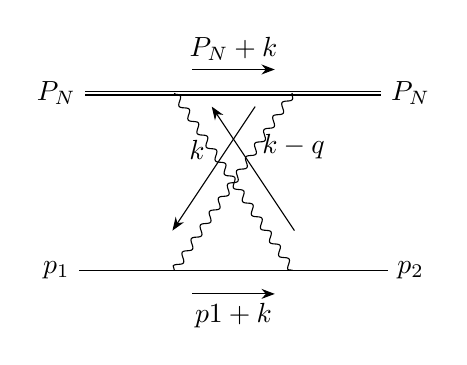
\begin{tikzpicture}[baseline=($(a)!0.5!(c)$)]
		\begin{feynman}
			\diagram[horizontal=i1 to f1,layered layout,medium]{
			i1[particle=$P_N$] -- [double distance=1pt] a -- [double distance=1pt,momentum=$P_N+k$] b -- [double distance=1pt] f1[particle=$P_N$],
			i2[particle=$p_1$] -- [] c -- [momentum'=$p1+k$] d -- [] f2[particle=$p_2$],
			{ [same layer] a --[draw=none] c},
			{ [same layer] b-- [draw=none] d},
			};
			\diagram*{
			(a) -- [photon,rmomentum=$k-q$] (d),
			(b) -- [photon,momentum'=$k$] (c),
			};
		\end{feynman}
	\end{tikzpicture}
	+
	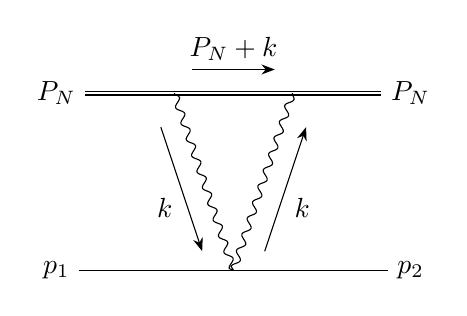
\begin{tikzpicture}[baseline=($(a)!0.5!(c)$)]
		\begin{feynman}
			\diagram[horizontal=i1 to f1,layered layout,medium]{
			i1[particle=$P_N$] -- [double distance=1pt] a -- [double distance=1pt,momentum=$P_N+k$] b -- [double distance=1pt] f1[particle=$P_N$],
			i2[particle=$p_1$] -- [] c -- [] d -- [] f2[particle=$p_2$],
			{ [same layer] a --[draw=none] c},
			{ [same layer] b-- [draw=none] d},
			};
			\vertex at ($(c)!0.5!(d)$) (f);
			\diagram*{
			(a) -- [photon,momentum'=$k$] (f),
			(b) -- [photon,rmomentum=$k$] (f),
			};
		\end{feynman}
	\end{tikzpicture}
\end{align*}
\begin{align*}
	\feynmandiagram[horizontal=i1 to f1,layered layout,inline=($(a)!0.5!(c)$),medium]{
	i1[particle=$P_N$] -- [double distance=1pt] a -- [double distance=1pt,momentum=$P_N-k^0$] b -- [double distance=1pt] f1[particle=$P_N$],
	i2[particle=$p_1$] -- [] c -- [momentum=$p_1+k$] d -- [] f2[particle=$p_2$],
	{ [same layer] a -- [photon,momentum'=$k$] c},
	{ [same layer] b -- [photon,rmomentum=$k-q$] d},
	};=-e^2v^{0}\int\frac{\dd^4k}{(2\pi)^4}\frac{i}{\vb{k}^2}\frac{}{}<+content+>
\end{align*}<++>
\begin{align*}
	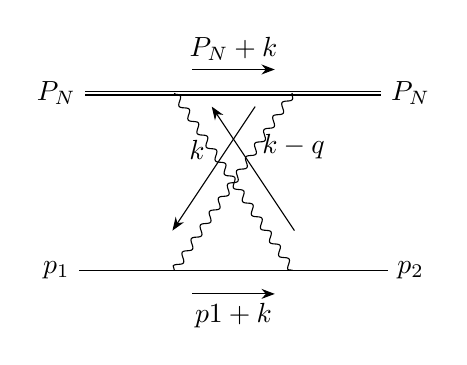
\begin{tikzpicture}[baseline=($(a)!0.5!(c)$)]
		\begin{feynman}
			\diagram[horizontal=i1 to f1,layered layout,medium]{
			i1[particle=$P_N$] -- [double distance=1pt] a -- [double distance=1pt,momentum=$P_N+k$] b -- [double distance=1pt] f1[particle=$P_N$],
			i2[particle=$p_1$] -- [] c -- [momentum'=$p1+k$] d -- [] f2[particle=$p_2$],
			{ [same layer] a --[draw=none] c},
			{ [same layer] b-- [draw=none] d},
			};
			\diagram*{
			(a) -- [photon,rmomentum=$k-q$] (d),
			(b) -- [photon,momentum'=$k$] (c),
			};
		\end{feynman}
	\end{tikzpicture} <+content+>
\end{align*}<++>
\begin{align*}
	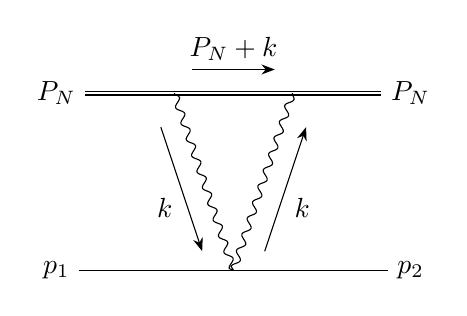
\begin{tikzpicture}[baseline=($(a)!0.5!(c)$)]
		\begin{feynman}
			\diagram[horizontal=i1 to f1,layered layout,medium]{
			i1[particle=$P_N$] -- [double distance=1pt] a -- [double distance=1pt,momentum=$P_N+k$] b -- [double distance=1pt] f1[particle=$P_N$],
			i2[particle=$p_1$] -- [] c -- [] d -- [] f2[particle=$p_2$],
			{ [same layer] a --[draw=none] c},
			{ [same layer] b-- [draw=none] d},
			};
			\vertex at ($(c)!0.5!(d)$) (f);
			\diagram*{
			(a) -- [photon,momentum'=$k$] (f),
			(b) -- [photon,rmomentum=$k$] (f),
			};
		\end{feynman}
	\end{tikzpicture}<+content+>
\end{align*}<++>
\subsubsection{SNRQED}\fi

\section{Local Operator and Matrix Element of Scalar NRQED}
Assuming the full theory of the scalar electron is scalar QED, we can mimic the effect of nucleus, or rather to say, Coulomb potential, with heavy scalar effective theory, as mentioned before. For simplicity, and also the goal of replicating divergence produced by Klein-Gordon equation, there's no need involving any other effect the nucleus might have. And as pionted out by Bodwin, Braaten and Lepage in 1995\cite{Bodwin1995}, when discussing heavy quarkonium problem, non-relativistic Coulomb gauge wavefunction can be defined as NRQCD Bethe-Salpeter $Q\bar Q$ wavefunction, evaluated at equal time. As an analogy, we can define NRQED wavefunction in the same fashion. Therefore, we can describe the radial wavefunction in terms of a matrix element 
\begin{align}
	R(x)=\mel{0}{\psi(x)N(0)}{atom}.\label{wavefunction}
\end{align}
We think that the divergence of wavefunction comes from the non-local attribute of operator $\psi(x)N(0)$ rather than the state $\ket{atom}$ itself, so it can be analyzed by operator product expansion (OPE)\cite{Lepage:1997cs}. Therefore, we can transform the problem to another matrix element\footnote{Here the actual momentum of the nucleus is $P_N=m_Nv_N$ but since $m_N$ is decoupled in HSET, it can not appear anywhere in our calculations} (note that OPE is relations between operators, thus independent of where these operators are located at)
\begin{align}	
	\mel{0}{\psi(x)N(0)\tilde\psi(p)\tilde N(k)}{0}=\int\frac{\dd^4 p}{(2\pi)^4}\frac{\dd^4 k}{(2\pi)^4}e^{-ip\cdot y}e^{-ik\cdot z}\mel{0}{\psi(x)N(0)\psi(y)N(z)}{0}.\label{NLME}
\end{align}	

To reproduce the singular behavior of ``Klein-Gordon Hydrogen'' wavefunction near origin, we could try OPE. But the dependence of x in this non-local matrix element can also be taken as a regularization scheme and thus the result should be the same as local one
$$\mel{0}{\psi(0)N(0)\tilde\psi(p)\tilde N(k)}{0}$$
without renormalization (except for the choice of different regulators). And the logarithmic terms of x in \eqref{wavefunction} can be reproduced by the logarithmic divergence of local operators. From what we learned in the discussion of Klein-Gordon equation in quantum mechanics, we know that the wavefunction only contains logarithmic divergence at the origin so that's the only type of divergence we're looking for. In this section, we'll isolate the logarithmic divergence using dimensional regularization, and reproduce what we obtained in quantum mechanics perturbation theory. 

Intuitively, we can assume $\psi(x)$ is just the scalar field operator in scalar QED. But what we need is logarithmic divergence start at $Z^2\a^2$ order, and using relativistic scalar field operator will result in logarithmic divergence at $Z\a$ order, which, since we already know the answer to the question, is not what we want. However, since QED, or in our case, scalar QED, has no bound on how small the distance it can probe, we might observe that in order to investigate low energy physics, we can't use theory with such sensitivity in short range.

The alternative is to use scalar NRQED on the scalar electron side. Through it's a non-relativistic theory thus not the first chioce when studying a relativistic problem, the natural energy cutoff it provides will be very convenient in this problem.

First we define $\epsilon=3-d$ and on-shell momentum $P_N=m_Nv_N$, also the momentum of scalar electron is $p=(E,\vbp)$ and the momentum of nucleus is $P_N+k$.
\subsection{NLO}
It's obvious that the tree level has no divergence of any kind, so we'll start at one loop.

After dimensional regularization, the Gamma function in the numerator is something like $\Gamma(n-d/2)$ and Gamma function doesn't have pole at half integer. We can prove that any one-loop diagram involved does not have logarithmic divergence.
\begin{comment}
, for example
\begin{align*}
	  & \mel{0}{\psi_e(0)N(0)(-ie\mu^{-\epsilon})\int\dd^4y\bar\psi_e\psi_e A^0(-iZe\mu^{-\epsilon})\int\dd^4z\bar NNA^0}{0}=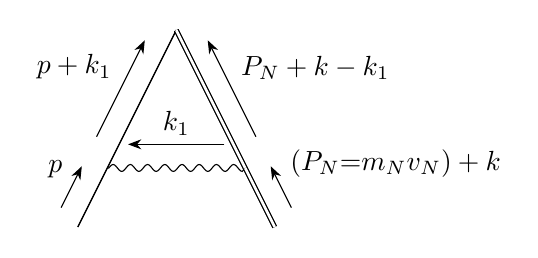
\begin{tikzpicture}[baseline=($(p1)!0.5!(x)$)]
		\begin{feynman}
			\vertex (p1);
			\vertex[right=2.5cm of p1] (p2);
			\vertex at ($(p1)!0.5!(p2)+(0,2.5cm)$) (x) ;
			\vertex at ($(p1)!0.3!(x)$) (y1);
			\vertex at ($(p2)!0.3!(x)$) (z1);
			%
			\diagram* {
			(p1) -- [] (x);
			(p2) -- [double distance=1pt] (x);
			(y1) -- [photon,rmomentum=$k_1$] (z1);
			(p1) -- [momentum=\(p\)] (y1);
			(p2) -- [momentum'=$(P_{N}\text{=}m_{N}v_{N})+k$,double distance=1pt] (z1);
			(y1) -- [momentum=\(p+k_1\)] (x);
			(z1) -- [momentum'=\(P_{N}+k-k_1\),double distance=1pt] (x);
			};
		\end{feynman}
	\end{tikzpicture}
\end{align*}
which doesn't have logarithmic divergence.
\end{comment}
\subsection{NNLO}
Since we're calculating Green function, the nucleus is off-shell by $k$. Although the effect is just a shift in electron energy (see Appendix \ref{appendix:contour}), it's convenient for us to redefine $E'=E+k^0$. 

All the Feynman rules we need are derived above except for one: on the top of the diagram, the joint point stands for composite operator $\psi(0)N(0)$, whose Feynman rule is just $1$; if it's seperated a little, it stands for non-local fields in operator product expansion and can be treated as a exponential factor $e^{-i \vbk \cdot \vb{x}}$ where $\vbk$ is the momentum of the cloest line in the electron side. 
\begin{align*}
	&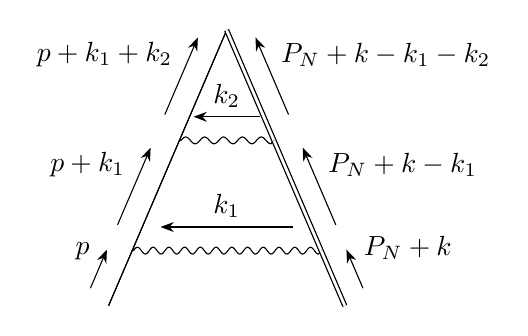
\begin{tikzpicture}[baseline=($(p1)!0.5!(x)$)]
		\begin{feynman}
			\vertex (p1);
			\vertex[right=3cm of p1] (p2);
			\vertex at ($(p1)!0.5!(p2)+(0,3.5cm)$) (x) ;
			\vertex at ($(p1)!0.2!(x)$) (y1);
			\vertex at ($(p2)!0.2!(x)$) (z1);
			\vertex at ($(p1)!0.6!(x)$) (y2);
			\vertex at ($(p2)!0.6!(x)$) (z2);
			%
			\diagram* {
			(p1) -- [] (x);
			(p2) -- [double distance=1pt] (x);
			(y1) -- [photon,rmomentum=$k_1$] (z1);
			(y2) -- [photon,rmomentum=$k_2$] (z2);
			(p1) -- [momentum=\(p\)] (y1);
			(p2) -- [momentum'=$P_{N}+k$,double distance=1pt] (z1);
			(y1) -- [momentum=\(p+k_1\)] (y2);
			(z1) -- [momentum'=\(P_{N}+k-k_1\),double distance=1pt] (z2);
			(y2) -- [momentum=\(p+k_1+k_2\)] (x);
			(z2) -- [momentum'=\(P_{N}+k-k_1-k_2\),double distance=1pt] (x);
			};
		\end{feynman}
	\end{tikzpicture}\\ =&-\mu^{2\epsilon}Z^2e^4\bqty{\int\frac{[dk_1]}{\vb{\abs{k_1}}^2}\frac{[dk_2]}{\vb{\abs{k_2}}^2}\frac{1}{k^0-k_1^0-k_2^0+i\epsilon}\frac{1}{k^0-k_1^0+i\epsilon}\frac{1}{E+k_1^0-\frac{\vb{(p+k_1)}^2}{2m}+i\epsilon}\frac{1}{E+k_1^0+k_2^0-\frac{\vb{(p+k_1+k_2)}^2}{2m}+i\epsilon}}
	\\
	\intertext{integrate out the temporal component of loop momentum, then perform shifts $\vbk_1\rightarrow\vbk_1-\vbp$ and $\vbk_2\rightarrow\vbk_2-\vbk_1-\vbp$ on them}
	=&\mu^{2\epsilon}Z^2e^4\bqty{\int\frac{\dd^d\vb{k_1}}{(2\pi)^d}\frac{\dd^d\vb{k_2}}{(2\pi)^d}\frac{1}{\vb{\abs{k_1-p}}^2}\frac{1}{\vb{\abs{k_2-k_1}}^2}\frac{1}{E'-\frac{\vb{\abs{k_1}}^2}{2m}+2i\epsilon}\frac{1}{E'-\frac{\vb{\abs{k_2}}^2}{2m}+2i\epsilon}}\\
	=&4m^2Z^2\alpha ^2 \mu^{2\epsilon}\int_0^1\dd x_1\dd x_2\delta (x_1 +x_2-1)
	\int\frac{\dd^d\vb{k_1}}{(2\pi)^d}\frac{1}{\vb{\abs{k_1-p}}^2}\frac{1}{[\vb{\abs{k_1}}^2-2mE']^2}\frac{1}{\left(\vbk_1^2-\frac{2 mE }{x_1}\right)^{2-d/2}	}\\&
	\bqty{ 2^{4-d} \pi ^{2-\frac{d}{2}} \left(x_1-x_1^2\right)^{\frac{d}{2}-2} \Gamma \left(2-\frac{d}{2}\right)}\\
	=&4m^2Z^2 \alpha ^2\mu^{2\epsilon}\int_0^1\dd x_1\dd x_2\dd y_1\dd y_2\dd y_3 \delta (x_1 +x_2-1) \delta (y_1+y_2+y_3-1)   \frac{2^{4-2 d} \pi ^{2-d} \left(x_1 -x_1 ^2\right)^{\frac{d}{2}-2} y_3^{1-\frac{d}{2}} \Gamma (4-d)}{\left(p^2 y_1-p^2 y_1^2-\frac{2m E  y_3}{ x_1 }-2 m E y_2\right)^{4-d}}\\
	=&\text{finite terms}
\end{align*}
Actually, after integrated the temporal part, we can determine from superficial divergence that unless the power of the numerator is higher than $\vbk^2$, the diagram can not be divergent. We can do so by adding relativistic corrections 
\begin{align*}
	& 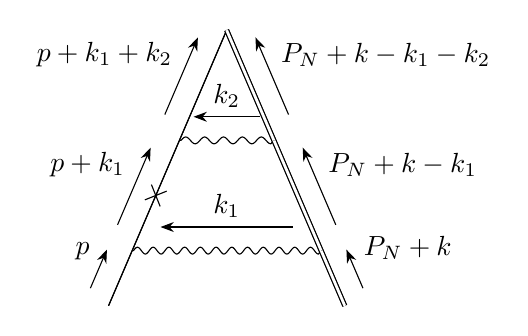
\begin{tikzpicture}[baseline=($(p1)!0.5!(x)$)]
		\begin{feynman}
			\vertex (p1);
			\vertex[right=3cm of p1] (p2);
			\vertex at ($(p1)!0.5!(p2)+(0,3.5cm)$) (x) ;
			\vertex at ($(p1)!0.2!(x)$) (y1);
			\vertex at ($(p2)!0.2!(x)$) (z1);
			\vertex at ($(p1)!0.6!(x)$) (y2);
			\vertex at ($(p2)!0.6!(x)$) (z2);
			\vertex at ($(y1)!0.5!(z1)$) (t);
			%
			\diagram* {
			(p1) -- [] (x);
			(p2) -- [double distance=1pt] (x);
			(y1) -- [photon,rmomentum=$k_1$] (z1);
			(y2) -- [photon,rmomentum=$k_2$] (z2);
			(p1) -- [momentum=\(p\)] (y1);
			(p2) -- [momentum'=$P_{N}+k$,double distance=1pt] (z1);
			(y1) -- [momentum=\(p+k_1\),insertion=0.5] (y2);
			(z1) -- [momentum'=\(P_{N}+k-k_1\),double distance=1pt] (z2);
			(y2) -- [momentum=\(p+k_1+k_2\)] (x);
			(z2) -- [momentum'=\(P_{N}+k-k_1-k_2\),double distance=1pt] (x);
			};
		\end{feynman}
	\end{tikzpicture}\\ =&-\mu^{2\epsilon}Z^2e^4\bqty{\int\frac{[dk_1]}{\vb{\abs{k_1}}^2}\frac{[dk_2]}{\vb{\abs{k_2}}^2}\frac{1}{k^0-k_1^0-k_2^0+i\epsilon}\frac{1}{k^0-k_1^0+i\epsilon}\frac{(\vbp+\vbk_1)^4/8m^3}{\bqty{E+k_1^0-\frac{\vb{(p+k_1)}^2}{2m}+i\epsilon}^2}\frac{1}{E+k_1^0+k_2^0-\frac{\vb{(p+k_1+k_2)}^2}{2m}+i\epsilon}}\\
	=&4m^2\mu^{2\epsilon}Z^2e^4
	\int\frac{\dd^d\vb{k_1}}{(2\pi)^d}\frac{\dd^d\vb{k_2}}{(2\pi)^d}\frac{1}{\vb{\abs{k_1-p}}^2}\frac{1}{\vb{\abs{k_2-k_1}}^2}\frac{\vb{\abs{k_1}}^4/4m^2}{[\vb{\abs{k_1}}^2-2mE']^2}\frac{1}{\vb{\abs{k_2}}^2-2mE'}\\
	\intertext{after integrated $\vbk_2$, the integral becomes}
	=&4m^2\mu^{2\epsilon}
	\int\frac{\dd^d\vb{k_1}}{(2\pi)^d}\frac{1}{\vb{\abs{k_1-p}}^2}\frac{\vb{\abs{k_1}}^4/4m^2}{[\vb{\abs{k_1}}^2-2mE']^2}\frac{1}{\left(\vbk_1^2-\frac{2 mE' }{x_1}\right)^{2-d/2}	}
	\bqty{\alpha ^2 2^{4-d} \pi ^{2-\frac{d}{2}}Z^2 \Gamma \left(2-\frac{d}{2}\right)\left(x_1-x_1^2\right)^{\frac{d}{2}-2}}\\
	=&Z^2\alpha ^2\mu^{2\epsilon}\int_0^1\dd x_1\dd x_2\dd y_1\dd y_2\dd y_3 \delta (x_1 +x_2-1) \delta (y_1+y_2+y_3-1)  \\
	&\Bigg\{
	2^{4-2 d} \pi ^{2-d} p^4 y_1^4 y_2 \left(x_1-x_1^2\right)^{\frac{d}{2}-2} y_3^{1-\frac{d}{2}} \Gamma (5-d) \left(\frac{1}{\frac{2 E' m x_2 y_3}{(x_1-1) x_1}-2 E' m y_2+p^2 \left(-y_1^2\right)+p^2 y_1}\right)^{5-d}\\&
	+\frac{2^{5-2 d} \pi ^{2-d} p^2 y_1^2 y_2 \left(x_1-x_1^2\right)^{\frac{d}{2}-2} y_3^{1-\frac{d}{2}} \Gamma (4-d) \Gamma \left(\frac{d}{2}+1\right) }{\Gamma \left(\frac{d}{2}\right)}\left(\frac{1}{\frac{2 E' m x_2 y_3}{(x_1-1) x_1}-2 E' m y_2+p^2 \left(-y_1^2\right)+p^2 y_1}\right)^{4-d}\\&
	+\frac{2^{6-2 d} \pi ^{2-d} p^2 y_1^2 y_2 \left(x_1-x_1^2\right)^{\frac{d}{2}-2} y_3^{1-\frac{d}{2}} \Gamma (4-d) \Gamma \left(\frac{d}{2}+1\right) }{ \Gamma \left(\frac{d}{2}\right )d}\left(\frac{1}{\frac{2 E' m x_2 y_3}{(x_1-1) x_1}-2 E' m y_2+p^2 \left(-y_1^2\right)+p^2 y_1}\right)^{4-d}\\&
	+\frac{2^{4-2 d} \pi ^{2-d} y_2 \left(x_1-x_1^2\right)^{\frac{d}{2}-2} y_3^{1-\frac{d}{2}} \Gamma (3-d) \Gamma \left(\frac{d}{2}+2\right) }{\Gamma \left(\frac{d}{2}\right)}\left(\frac{1}{\frac{2 E' m x_2 y_3}{(x_1-1) x_1}-2 E' m y_2+p^2 \left(-y_1^2\right)+p^2 y_1}\right)^{3-d}
		\Bigg\}\\
		\intertext{finish the integration of Feynman parameters, we have}
	= & Z^2\a^2(\frac{1}{2(3-d)}+\log \mu)+\text{finite terms}
\end{align*}
\begin{align*}
	& 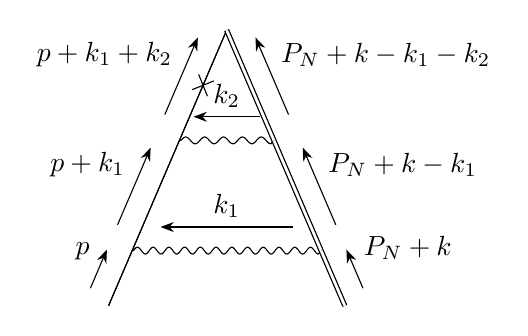
\begin{tikzpicture}[baseline=($(p1)!0.5!(x)$)]
		\begin{feynman}
			\vertex (p1);
			\vertex[right=3cm of p1] (p2);
			\vertex at ($(p1)!0.5!(p2)+(0,3.5cm)$) (x) ;
			\vertex at ($(p1)!0.2!(x)$) (y1);
			\vertex at ($(p2)!0.2!(x)$) (z1);
			\vertex at ($(p1)!0.6!(x)$) (y2);
			\vertex at ($(p2)!0.6!(x)$) (z2);
			\vertex at ($(y1)!0.5!(z1)$) (t);
			%
			\diagram* {
			(p1) -- [] (x);
			(p2) -- [double distance=1pt] (x);
			(y1) -- [photon,rmomentum=$k_1$] (z1);
			(y2) -- [photon,rmomentum=$k_2$] (z2);
			(p1) -- [momentum=\(p\)] (y1);
			(p2) -- [momentum'=$P_{N}+k$,double distance=1pt] (z1);
			(y1) -- [momentum=\(p+k_1\)] (y2);
			(z1) -- [momentum'=\(P_{N}+k-k_1\),double distance=1pt] (z2);
			(y2) -- [momentum=\(p+k_1+k_2\),insertion=0.5] (x);
			(z2) -- [momentum'=\(P_{N}+k-k_1-k_2\),double distance=1pt] (x);
			};
		\end{feynman}
	\end{tikzpicture}\\ =&-\mu^{2\epsilon}Z^2e^4\bqty{\int\frac{[dk_1]}{\vb{\abs{k_1}}^2}\frac{[dk_2]}{\vb{\abs{k_2}}^2}\frac{1}{k^0-k_1^0-k_2^0+i\epsilon}\frac{1}{k^0-k_1^0+i\epsilon}\frac{1}{E+k_1^0-\frac{\vb{(p+k_1)}^2}{2m}+i\epsilon}\frac{(\vbp+\vbk_2)^4/8m^3}{\bqty{E+k_1^0+k_2^0-\frac{\vb{(p+k_1+k_2)}^2}{2m}+i\epsilon}^2}}\\
	=&4m^2
	\mu^{2\epsilon}Z^2e^4\int\frac{\dd^d\vb{k_1}}{(2\pi)^d}\frac{\dd^d\vb{k_2}}{(2\pi)^d}\frac{1}{\vb{\abs{k_1-p}}^2}\frac{1}{\vb{\abs{k_2-k_1}}^2}\frac{1}{\vb{\abs{k_1}}^2-2mE'}\frac{\vb{\abs{k_2}}^4/4m^2}{[\vb{\abs{k_2}}^2-2mE']^2}\\
	=&
	\mu^{2\epsilon}Z^2e^4\int\frac{\dd^d\vb{k_1}}{(2\pi)^d}\frac{\dd^d\vb{k_2}}{(2\pi)^d}\frac{1}{\vb{\abs{k_1-p}}^2}\frac{1}{\vb{\abs{k_2-k_1}}^2}\frac{1}{\vb{\abs{k_1}}^2-2mE'}
	\Bqty{1+\frac{4mE'}{\vb{\abs{k_2}}^2-2mE'}+\frac{(2mE')^2}{[\vb{\abs{k_2}}^2-2mE']^2}}\\
	\intertext{only the highest order of $\vbk_2$ in the polynomial can contribute to the divergence, other terms are finite and can be dropped in the following calculations. This can be observed by simply counting the superficial divergence. Then one could find that by shifting $\vbk_2$ this integral becomes scaleless, thus zero under dimensional regularization}		
	%=& Z^2 \alpha ^2
	%\mu^{2\epsilon} 2^{4-d} \pi ^{2-\frac{d}{2}}\Gamma \left(3-\frac{d}{2}\right) 
	%\int_0^1\dd x_1\dd x_2\dd x_3\delta (x_1+x_2+x_3-1) \left(\frac{1}{x_1-x_1^2}\right)^{3-\frac{d}{2}}\\
	%&\int\frac{\dd^d\vb{k_2}}{(2\pi)^d}\left(\frac{1}{\vbk_2^2+\frac{2 x_2 \vbk_2\cdot \vbp}{x_1-1}+\frac{2 E' m x_3}{(x_1-1) x_1}+\frac{p^2 x_2^2}{(x_1-1) x_1}+\frac{p^2 x_2}{x_1-x_1^2}}\right)^{3-\frac{d}{2}}\\
	= & 0+\text{finite terms.}
\end{align*}
We can see that the total divergence is $$Z^2\a^2\pqty{\frac{1}{2(3-d)}+\log \mu}.$$

Comparing the final result of divergence between OPE and QM wavefunctions, we can see that the coefficient of $\log{\mu}$ is consistent with which of the logarithm divergence in the asymptotic behavior of Klein-Gordon wavefunction and Schr\"odinger wavefunction with relativistic correction.

\section{Operator Product Expansion and Explicitly Coordinate-dependent Divergence}
Now that we have successfully isolated the logarithmic divergence of local operators, we can calculate the coordinate-dependent divergence that we actually encountered regarding the wavefunction. As mentioned before, we can achieve that via OPE. 

The operator product expansion\cite{Collins1984} (OPE) is to write the products of several local operators evaluated at different points, in the limit of those points approaching each other, as a series of composite local operators, i.e.
\begin{align}
	\mathcal{O}_1(x)\mathcal{O}_2(y)=\sum_nC_n(x-y)\mathcal{O}_n(x)
\end{align}
In our case, the equation becomes
\begin{align}
	\psi(x)N(0)=C_0(x)\psi(0)N(0)+\sum_nC_n(x)\mathcal{O}_n(0)\label{OPE}
\end{align}
The logarithmic divergence, which is the highest order of divergence on the left hand side, only appears in the coefficient of the first term in the right hand side. Since it's an equation for operators, we can also write it down as matrix elements
\begin{align}
	\mel{0}{\psi(x)N(0)}{0}=C_0(x)\psi(0)N(0)+\sum_nC_n(x)\mathcal{O}_n(0)\label{OPEME}
\end{align}
The matrix element $\mel{0}{\psi(0)N(0)}{0}$, is exactly what we calculated in the last section. 

For any type of diagrams on the left hand side of equation \eqref{OPEME}, we have
\begin{align}
	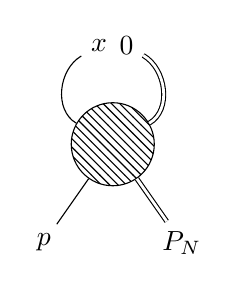
\begin{tikzpicture}[baseline=($(p1)!0.5!(x)$)]
		\tikzfeynmanset{
			my blob/.style={
					/tikzfeynman/blob,
					/tikz/minimum size=30pt,
				},
			%every vertex/.style={my blob},
		}
		\begin{feynman}
			\vertex (p1) {$p$};
			\vertex[right=1.75cm of p1] (p2) {$P_N$};
			\vertex at ($(p1)!0.4!(p2)+(0,2.5cm)$) (x) {$x$};
			\vertex at ($(p1)!0.6!(p2)+(0,2.5cm)$) (0) {$0$};
			\vertex at ($(p1)!0.5!(x)$) (y1);
			\vertex at ($(p2)!0.5!(0)$) (z1);
			\vertex at ($(y1)!0.5!(z1)$) (o);
			\node[my blob] at (o) (o1);
			%
			\diagram* {
			(p1) --  (o1);
			(p2) -- [double distance=1pt] (o1);
			%(y1) -- [photon,rmomentum=$k_1$] (z1);
			%(p1) -- [] (y1);
			%(p2) -- [double distance=1pt] (z1);
			(o1) -- [out=150, in=210] (x);
			(o1) -- [out=30, in=330,double distance=1pt] (0);
			};
		\end{feynman}
	\end{tikzpicture}
	=
	\bqty{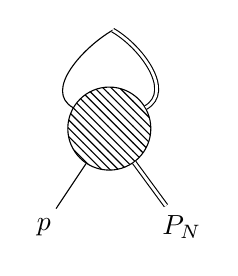
\begin{tikzpicture}[baseline=($(p1)!0.5!(x)$)]
			\tikzfeynmanset{
				my blob/.style={
						/tikzfeynman/blob,
						/tikz/minimum size=30pt,
					},
				%every vertex/.style={my blob},
			}
			\begin{feynman}
				\vertex (p1) {$p$};
				\vertex[right=1.75cm of p1] (p2) {$P_N$};
				\vertex at ($(p1)!0.4!(p2)+(0,2.5cm)$) (x) ;
				\vertex at ($(p1)!0.5!(p2)+(0,2.5cm)$) (0) ;
				\vertex at ($(p1)!0.5!(x)$) (y1);
				\vertex at ($(p2)!0.5!(0)$) (z1);
				\vertex at ($(y1)!0.5!(z1)$) (o);
				\node[my blob] at (o) (o1);
				%
				\diagram* {
				(p1) --  (o1);
				(p2) -- [double distance=1pt] (o1);
				%(y1) -- [photon,rmomentum=$k_1$] (z1);
				%(p1) -- [] (y1);
				%(p2) -- [double distance=1pt] (z1);
				(o1) -- [out=150, in=210] (0);
				(o1) -- [out=30, in=330,double distance=1pt] (0);
				};
			\end{feynman}
		\end{tikzpicture}-UV}
	+
	\bqty{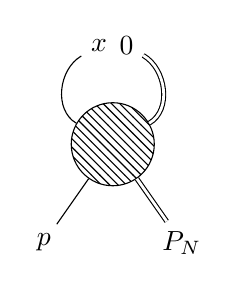
\begin{tikzpicture}[baseline=($(p1)!0.5!(x)$)]
			\tikzfeynmanset{
				my blob/.style={
						/tikzfeynman/blob,
						/tikz/minimum size=30pt,
					},
				%every vertex/.style={my blob},
			}
			\begin{feynman}
				\vertex (p1) {$p$};
				\vertex[right=1.75cm of p1] (p2) {$P_N$};
				\vertex at ($(p1)!0.4!(p2)+(0,2.5cm)$) (x) {$x$};
				\vertex at ($(p1)!0.6!(p2)+(0,2.5cm)$) (0) {$0$};
				\vertex at ($(p1)!0.5!(x)$) (y1);
				\vertex at ($(p2)!0.5!(0)$) (z1);
				\vertex at ($(y1)!0.5!(z1)$) (o);
				\node[my blob] at (o) (o1);
				%
				\diagram* {
				(p1) --  (o1);
				(p2) -- [double distance=1pt] (o1);
				%(y1) -- [photon,rmomentum=$k_1$] (z1);
				%(p1) -- [] (y1);
				%(p2) -- [double distance=1pt] (z1);
				(o1) -- [out=150, in=210] (x);
				(o1) -- [out=30, in=330,double distance=1pt] (0);
				};
			\end{feynman}
		\end{tikzpicture}-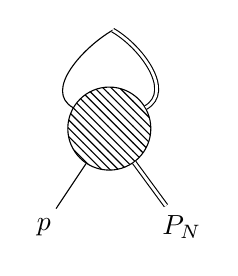
\begin{tikzpicture}[baseline=($(p1)!0.5!(x)$)]
			\tikzfeynmanset{
				my blob/.style={
						/tikzfeynman/blob,
						/tikz/minimum size=30pt,
					},
				%every vertex/.style={my blob},
			}
			\begin{feynman}
				\vertex (p1) {$p$};
				\vertex[right=1.75cm of p1] (p2) {$P_N$};
				\vertex at ($(p1)!0.4!(p2)+(0,2.5cm)$) (x) ;
				\vertex at ($(p1)!0.5!(p2)+(0,2.5cm)$) (0) ;
				\vertex at ($(p1)!0.5!(x)$) (y1);
				\vertex at ($(p2)!0.5!(0)$) (z1);
				\vertex at ($(y1)!0.5!(z1)$) (o);
				\node[my blob] at (o) (o1);
				%
				\diagram* {
				(p1) --  (o1);
				(p2) -- [double distance=1pt] (o1);
				%(y1) -- [photon,rmomentum=$k_1$] (z1);
				%(p1) -- [] (y1);
				%(p2) -- [double distance=1pt] (z1);
				(o1) -- [out=150, in=210] (0);
				(o1) -- [out=30, in=330,double distance=1pt] (0);
				};
			\end{feynman}
		\end{tikzpicture}+UV}
\end{align}
where $UV$ stands for the ultraviolet divergent part in the local matrix elements. So by using our previous results, we only have to compute the second term, which is in fact a Fourier transformation.

In previous discussion, we mentioned that the small distance between two field operators in OPE can be treated as a regularization scheme, so we can safely assume that only OPE diagrams correspondent with logarithmic divergent local operator diagrams contains $\log x$ terms. Therefore, in this case, only one diagram is considered. Here we'll jump to the 3-dimension integral without temporal component (for details about involved contour integral, see Appendix \ref{appendix:contour}). 
\begin{align*}
	  & 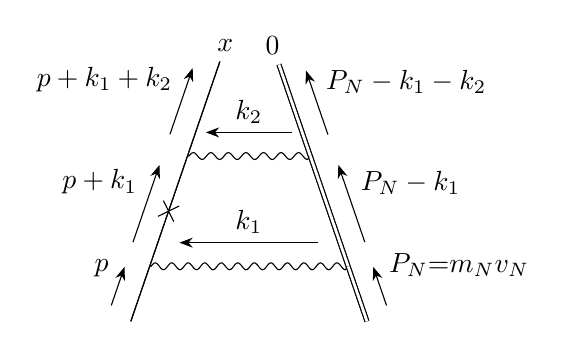
\begin{tikzpicture}[baseline=($(p1)!0.5!(x)$)]
		\begin{feynman}
			\vertex (p1);
			\vertex[right=3cm of p1] (p2);
			\vertex at ($(p1)!0.4!(p2)+(0,3.5cm)$) (x) {$x$};
			\vertex at ($(p1)!0.6!(p2)+(0,3.5cm)$) (0) {$0$};
			\vertex at ($(p1)!0.2!(x)$) (y1);
			\vertex at ($(p2)!0.2!(0)$) (z1);
			\vertex at ($(p1)!0.6!(x)$) (y2);
			\vertex at ($(p2)!0.6!(0)$) (z2);
			%
			\diagram* {
			(p1) -- [] (x);
			(p2) -- [double distance=1pt] (0);
			(y1) -- [photon,rmomentum=$k_1$] (z1);
			(y2) -- [photon,rmomentum=$k_2$] (z2);
			(p1) -- [momentum=\(p\)] (y1);
			(p2) -- [momentum'=$P_{N}\text{=}m_{N}v_{N}$,double distance=1pt] (z1);
			(y1) -- [momentum=\(p+k_1\),insertion=0.5] (y2);
			(z1) -- [momentum'=\(P_{N}-k_1\),double distance=1pt] (z2);
			(y2) -- [momentum=\(p+k_1+k_2\)] (x);
			(z2) -- [momentum'=\(P_{N}-k_1-k_2\),double distance=1pt] (0);
			};
		\end{feynman}
	\end{tikzpicture}-
	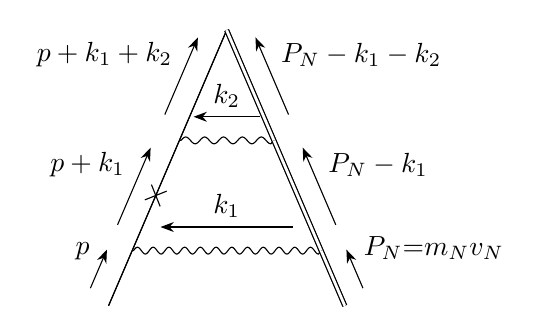
\begin{tikzpicture}[baseline=($(p1)!0.5!(x)$)]
		\begin{feynman}
			\vertex (p1);
			\vertex[right=3cm of p1] (p2);
			\vertex at ($(p1)!0.5!(p2)+(0,3.5cm)$) (x) ;
			\vertex at ($(p1)!0.2!(x)$) (y1);
			\vertex at ($(p2)!0.2!(x)$) (z1);
			\vertex at ($(p1)!0.6!(x)$) (y2);
			\vertex at ($(p2)!0.6!(x)$) (z2);
			\vertex at ($(y1)!0.5!(z1)$) (t);
			%
			\diagram* {
			(p1) -- [] (x);
			(p2) -- [double distance=1pt] (x);
			(y1) -- [photon,rmomentum=$k_1$] (z1);
			(y2) -- [photon,rmomentum=$k_2$] (z2);
			(p1) -- [momentum=\(p\)] (y1);
			(p2) -- [momentum'=$P_{N}\text{=}m_{N}v_{N}$,double distance=1pt] (z1);
			(y1) -- [momentum=\(p+k_1\),insertion=0.5] (y2);
			(z1) -- [momentum'=\(P_{N}-k_1\),double distance=1pt] (z2);
			(y2) -- [momentum=\(p+k_1+k_2\)] (x);
			(z2) -- [momentum'=\(P_{N}-k_1-k_2\),double distance=1pt] (x);
			};
		\end{feynman}
	\end{tikzpicture}\\
	= & 4m^2\mu^{2\epsilon}Z^2e^4
	\int\frac{\dd^d\vb{k_1}}{(2\pi)^d}\frac{\dd^d\vb{k_2}}{(2\pi)^d}\bqty{e^{-i\vb{k}_2\cdot\vb{x}}-1}\frac{1}{\vb{\abs{k_1-p}}^2}\frac{1}{\vb{\abs{k_2-k_1}}^2}\frac{\vb{\abs{k_1}}^4/4m^2}{[\vb{\abs{k_1}}^2-2mE']^2}\frac{1}{\vb{\abs{k_2}}^2-2mE'}\numberthis\label{tempformminus}\\
	= & 4m^2\mu^{2\epsilon}Z^2e^4\int_0^1\dd x_1\dd x_2\dd x_3\delta(1-x_1-x_2-x_3)
	\int\frac{\dd^d\vb{k_2}}{(2\pi)^d}\bqty{e^{-i\vb{k}_2\cdot\vb{x}}-1}\frac{1}{\vb{\abs{k_2}}^2-2mE'}\\&
	\frac{3 x_3 \left(\vbk_2^4 x_2^4+2 \vbk_2^2 \vbp^2 x_2^2 x_1^2+4 \vbk_2^2 x_2^3 x_1 \vbk_2\cdot\vbp+4 \vbp^2 x_2 x_1^3 \vbk_2\cdot\vbp+4 x_2^2 x_1^2 (\vbk_2\cdot\vbp)^2+\vbp^4 x_1^4\right)}{32 \pi }\\&
	\left(\frac{1}{\vbk_2^2 x_2-(-\vbk_2 x_2-\vbp x_1)^2-2 E m x_3+\vbp^2 x_1}\right)^{5/2}+\frac{3 x_3 \left(\frac{10}{3} \vbk_2^2 x_2^2+\frac{20}{3} x_2 x_1 \vbk_2\cdot\vbp+\frac{10}{3} \vbp^2 x_1^2\right)}{32 \pi } \\&
	\left(\frac{1}{\vbk_2^2 x_2-(-\vbk_2 x_2-\vbp x_1)^2-2 E m x_3+\vbp^2 x_1}\right)^{3/2}+\frac{15 x_3 }{32 \pi }\sqrt{\frac{1}{\vbk_2^2 x_2-(-\vbk_2 x_2-\vbp x_1)^2-2 E m x_3+\vbp^2 x_1}}
\end{align*}

\begin{appendices}
	\section{Useful formulas in Feynman integrals}
	Feynman parametrization used here is
	\begin{align}
		\frac{1}{\prod A_i^{d_i}}=\int\prod \dd x_i \delta(\sum x_i-1)\frac{\prod x_i^{d_i-1}}{\bqty{\sum x_iA_i}^{\sum d_i}}\frac{\Gamma(\sum d_i)}{\prod\Gamma(d_i)}
		\label{FEYNMANPARA}
	\end{align}
	Schwinger parametrization will also be useful
	\begin{align}
		\frac{1}{A^n}=\frac{1}{\Gamma{(n)}}\int_0^\infty\dd z z^{n-1}e^{-zA}
	\end{align}
	For arbitary one loop diagram of the following form, we have
	\begin{subequations} \label{1loopgamma}
		\begin{align}
			\int\frac{\dd^dk}{(2\pi)^d}\frac{k^{2\b}}{(k^2+\Delta)^n}
			  & =\frac{1}{(4\pi)^{n-\b}}\frac{\Gamma(\b+d/2)}{\Gamma(d/2)}\frac{\Gamma(n-\b-d/2)}{\Gamma(n)}\pqty{\frac{4\pi}{\Delta}}^{n-\b-d/2} \\
			  & =\frac{1}{(4\pi)^{d/2}}\frac{\Gamma(\b+d/2)}{\Gamma(d/2)}\frac{\Gamma(n-\b-d/2)}{\Gamma(n)}\pqty{\frac{1}{\Delta}}^{n-\b-d/2}
		\end{align}
	\end{subequations}
	where $\frac{1}{(4\pi)^{d/2}}$ often appears as $2^{-d}\pi^{-d/2}$.
	%  For two loop diagrams of this form ($\epsilon=3-d$)
	%  \begin{align}
	%	\mu^{-4\epsilon}\int\frac{\dd^d\vb{k}_1}{(2\pi)^d}\frac{\dd^d\vb{k}_2}{(2\pi)^d}\frac{1}{\vb{(k_1-a)}^2}\frac{1}{\vb{(k_2-k_1)}^2}\frac{\vbk_1^{2\a}}{(\vb{k}_1^2-c)^m}\frac{\vbk_2^{2\b}}{(\vb{k}_2^2-d)^n}
	%	\label{int}
	%  \end{align}
	%  The integral is evaluated to
	%  \begin{align*}
	%	&\mu^{-4\epsilon}\int_0^1\prod_{i=1}^2\dd x_i\delta(\sum x_i-1)\prod x_i^{d_i-1}\frac{\Gamma(n+1)}{\Gamma(n)}\frac{1}{(4\pi)^{n+1-\b}}\frac{\Gamma(\b+d/2)}{\Gamma(d/2)}\frac{\Gamma(n+1-\b-d/2)}{\Gamma(n+1)}\pqty{\frac{4\pi}{\a(x_i)}}^{n+1-\b-d/2}
	%	\\&\int\frac{\dd^d\vb{k}_1}{(2\pi)^d}\frac{1}{\vb{(k_1-a)}^2}\frac{\vbk_1^{2\a}}{(\vb{k}_1^2-c)^m}\frac{1}{(\vb{k}_1-\Delta_2)^{n+1-\b-d/2}}\\
	%	=&\mu^{-4\epsilon}\int_0^1\prod_{i=1}^2\dd x_i\delta(\sum x_i-1)\prod x_i^{d_i-1}\frac{1}{(4\pi)^{n+1-\b}}\frac{\Gamma(\b+d/2)}{\Gamma(d/2)}\frac{\Gamma(n+1-\b-d/2)}{\Gamma(n)}\pqty{\frac{4\pi}{\a(x_i)}}^{n+1-\b-d/2}\int_0^1\prod_{i=1}^3\dd y_j\delta(\sum y_j-1)
	%	\\&\prod y_j^{d_j-1}
	%	\frac{\Gamma(m+n+2-\b-d/2)}{\Gamma(m)\Gamma(n+1-\b-d/2)}\frac{1}{(4\pi)^{m+n+2-\a-\b-d/2}}\frac{\Gamma(\a+d/2)}{\Gamma(d/2)}\frac{\Gamma(m+n+2-\a-\b-d)}{\Gamma(m+n+2-\b-d/2)}\pqty{\frac{4\pi}{\Delta_1}}^{m+n+2-\a-\b-d}
	%	\\
	%	=&\mu^{-4\epsilon}\int_0^1\prod_{i=1}^2\dd x_i\delta(\sum x_i-1)\prod x_i^{d_i-1}\frac{1}{(4\pi)^{d}}\frac{\Gamma(\b+d/2)}{\Gamma(d/2)}\frac{1}{\Gamma(n)}\pqty{\frac{1}{\a(x_i)}}^{n+1-\b-d/2}
	%	\\&\int_0^1\prod_{i=1}^3\dd y_j\delta(\sum y_j-1)\prod y_j^{d_j-1}\frac{\Gamma(\a+d/2)}{\Gamma(d/2)}\frac{\Gamma(m+n+2-\a-\b-d)}{\Gamma(m)}\pqty{\frac{1}{\Delta_1}}^{m+n+2-\a-\b-d}
	% \end{align*}<++>
	\section{Contour Integral}
	\label{appendix:contour}
	If the nucleus is put on-shell, integral with the structure of the form
	\begin{align}
		\int[dk_1][dk_2]f(\vb{k}_1,\vb{k}_2)\frac{1}{-k_1^0-k_2^0+i\epsilon}\frac{1}{-k_1^0+i\epsilon}\frac{1}{[E+k_1^0-\vb{V}_2+i\epsilon]^m}\frac{1}{[E+k_1^0+k_2^0-\vb{V}_2+i\epsilon]^n}\label{pretemporal}
	\end{align}
	will always produce
	\begin{align}
		\int\frac{\dd^d\vb{k_1}}{(2\pi)^d}\frac{\dd^d\vb{k_2}}{(2\pi)^d}f(\vb{k}_1,\vb{k}_2)\frac{1}{[E-\vb{V}_1+2i\epsilon]^m}\frac{1}{[E-\vb{V}_2+2i\epsilon]^n}\label{halfgreen}
	\end{align}
	with $k_1^0$ and $k_2^0$ goes to zero.

	If the nucleus is slightly off-shell by $k$, there'll be a slight shift of energy in the non-relativistic propagators
	\begin{align*}
		  & \int[dk_1][dk_2]f(\vb{k}_1,\vb{k}_2)\frac{1}{-k_1^0-k_2^0+k^0+i\epsilon}\frac{1}{-k_1^0+k^0+i\epsilon}\frac{1}{[E+k_1^0-\vb{V}_2+i\epsilon]^m}\frac{1}{[E+k_1^0+k_2^0-\vb{V}_2+i\epsilon]^n} \\
		= & \int\frac{\dd^d\vb{k_1}}{(2\pi)^d}\frac{\dd^d\vb{k_2}}{(2\pi)^d}f(\vb{k}_1,\vb{k}_2)\frac{1}{[E+k^0-\vb{V}_1+2i\epsilon]^m}\frac{1}{[E+k^0-\vb{V}_2+2i\epsilon]^n}
	\end{align*}
	If we define $E'=E+k^0$, the structure falls back to \eqref{halfgreen}.

	One example is this Green function
	\begin{align*}
		  & 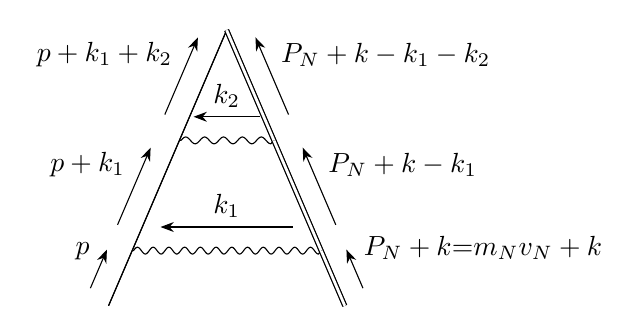
\begin{tikzpicture}[baseline=($(p1)!0.5!(x)$)]
			\begin{feynman}
				\vertex (p1);
				\vertex[right=3cm of p1] (p2);
				\vertex at ($(p1)!0.5!(p2)+(0,3.5cm)$) (x) ;
				\vertex at ($(p1)!0.2!(x)$) (y1);
				\vertex at ($(p2)!0.2!(x)$) (z1);
				\vertex at ($(p1)!0.6!(x)$) (y2);
				\vertex at ($(p2)!0.6!(x)$) (z2);
				%
				\diagram* {
				(p1) -- [] (x);
				(p2) -- [double distance=1pt] (x);
				(y1) -- [photon,rmomentum=$k_1$] (z1);
				(y2) -- [photon,rmomentum=$k_2$] (z2);
				(p1) -- [momentum=\(p\)] (y1);
				(p2) -- [momentum'=$P_{N}+k\text{=}m_{N}v_{N}+k$,double distance=1pt] (z1);
				(y1) -- [momentum=\(p+k_1\)] (y2);
				(z1) -- [momentum'=\(P_{N}+k-k_1\),double distance=1pt] (z2);
				(y2) -- [momentum=\(p+k_1+k_2\)] (x);
				(z2) -- [momentum'=\(P_{N}+k-k_1-k_2\),double distance=1pt] (x);
				};
			\end{feynman}
		\end{tikzpicture}\\ =&-\mu^{2\epsilon}Z^2e^4\bqty{\int\frac{[dk_1]}{\vb{\abs{k_1}}^2}\frac{[dk_2]}{\vb{\abs{k_2}}^2}\frac{1}{k^0-k_1^0-k_2^0+i\epsilon}\frac{1}{k^0-k_1^0+i\epsilon}\frac{1}{E+k_1^0-\frac{\vb{(p+k_1)}^2}{2m}+i\epsilon}\frac{1}{E+k_1^0+k_2^0-\frac{\vb{(p+k_1+k_2)}^2}{2m}+i\epsilon}}\\
		=&\mu^{2\epsilon}Z^2e^4\bqty{\int\frac{\dd^d\vb{k_1}}{(2\pi)^d}\frac{\dd^d\vb{k_2}}{(2\pi)^d}\frac{1}{\vb{\abs{k_1-p}}^2}\frac{1}{\vb{\abs{k_2-k_1}}^2}\frac{1}{E'-\frac{\vb{\abs{k_1}}^2}{2m}+2i\epsilon}\frac{1}{E'-\frac{\vb{\abs{k_2}}^2}{2m}+2i\epsilon}}\\
		=& 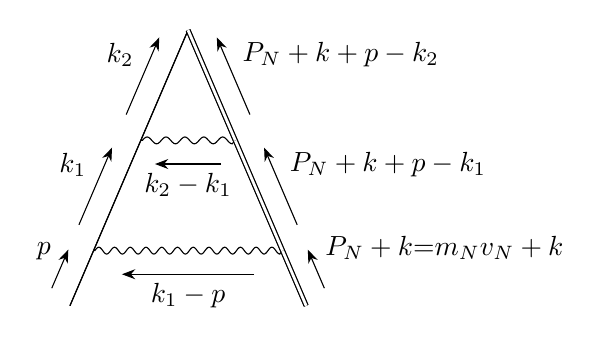
\begin{tikzpicture}[baseline=($(p1)!0.5!(x)$)]
			\begin{feynman}
				\vertex (p1);
				\vertex[right=3cm of p1] (p2);
				\vertex at ($(p1)!0.5!(p2)+(0,3.5cm)$) (x) ;
				\vertex at ($(p1)!0.2!(x)$) (y1);
				\vertex at ($(p2)!0.2!(x)$) (z1);
				\vertex at ($(p1)!0.6!(x)$) (y2);
				\vertex at ($(p2)!0.6!(x)$) (z2);
				%
				\diagram* {
				(p1) -- [] (x);
				(p2) -- [double distance=1pt] (x);
				(y1) -- [photon,rmomentum'=\(k_1-p\)] (z1);
				(y2) -- [photon,rmomentum'=\(k_2-k_1\)] (z2);
				(p1) -- [momentum=\(p\)] (y1);
				(p2) -- [momentum'=$P_{N}+k\text{=}m_{N}v_{N}+k$,double distance=1pt] (z1);
				(y1) -- [momentum=\(k_1\)] (y2);
				(z1) -- [momentum'=\(P_{N}+k+p-k_1\),double distance=1pt] (z2);
				(y2) -- [momentum=\(k_2\)] (x);
				(z2) -- [momentum'=\(P_{N}+k+p-k_2\),double distance=1pt] (x);
				};
			\end{feynman}
		\end{tikzpicture}
	\end{align*}
	As for any OPE diagram, it's just a regular local one multiplied by a exponential factor, and since we're choosing $x=(0,\vb{x})$, this factor can be included into $f(\vb{k}_1,\vb{k}_2)$ in \eqref{pretemporal}. That means it also becomes \eqref{halfgreen}. We also performed a momentum shift in the computation of regular local ones, what we did is basicly assign $\vbk_2$ to the upper photon line and after the contour integral, we reassign $\vbk_2$ to the upper electron line. Therefore the exponential factor will always becomes $e^{-i\vbk_2\cdot \vb{x}}$ in the end. 

	For example, 
	\begin{align*}
		& 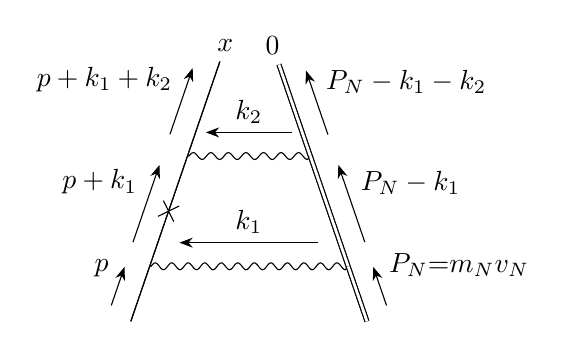
\begin{tikzpicture}[baseline=($(p1)!0.5!(x)$)]
			\begin{feynman}
				\vertex (p1);
				\vertex[right=3cm of p1] (p2);
				\vertex at ($(p1)!0.4!(p2)+(0,3.5cm)$) (x) {$x$};
				\vertex at ($(p1)!0.6!(p2)+(0,3.5cm)$) (0) {$0$};
				\vertex at ($(p1)!0.2!(x)$) (y1);
				\vertex at ($(p2)!0.2!(0)$) (z1);
				\vertex at ($(p1)!0.6!(x)$) (y2);
				\vertex at ($(p2)!0.6!(0)$) (z2);
				%
				\diagram* {
				(p1) -- [] (x);
				(p2) -- [double distance=1pt] (0);
				(y1) -- [photon,rmomentum=$k_1$] (z1);
				(y2) -- [photon,rmomentum=$k_2$] (z2);
				(p1) -- [momentum=\(p\)] (y1);
				(p2) -- [momentum'=$P_{N}\text{=}m_{N}v_{N}$,double distance=1pt] (z1);
				(y1) -- [momentum=\(p+k_1\),insertion=0.5] (y2);
				(z1) -- [momentum'=\(P_{N}-k_1\),double distance=1pt] (z2);
				(y2) -- [momentum=\(p+k_1+k_2\)] (x);
				(z2) -- [momentum'=\(P_{N}-k_1-k_2\),double distance=1pt] (0);
				};
			\end{feynman}
		\end{tikzpicture}\\=&
		-\mu^{2\epsilon}Z^2e^4\bqty{\int\frac{[dk_1]}{\vb{\abs{k_1}}^2}\frac{[dk_2]}{\vb{\abs{k_2}}^2}\frac{e^{-i(\vbp+\vbk_1+\vbk_2)\cdot \vb{x}}}{k^0-k_1^0-k_2^0+i\epsilon}\frac{1}{k^0-k_1^0+i\epsilon}\frac{(\vbp+\vbk_1)^4/8m^3}{\bqty{E+k_1^0-\frac{\vb{(p+k_1)}^2}{2m}+i\epsilon}^2}\frac{1}{E+k_1^0+k_2^0-\frac{\vb{(p+k_1+k_2)}^2}{2m}+i\epsilon}}\\
		=&\mu^{2\epsilon}Z^2e^4
		\int\frac{\dd^d\vb{k_1}}{(2\pi)^d}\frac{\dd^d\vb{k_2}}{(2\pi)^d}e^{-i(\vbp+\vbk_1+\vbk_2)\cdot \vb{x}}\frac{1}{\vb{\abs{k_1}}^2}\frac{1}{\vb{\abs{k_2}}^2}\frac{(\vbp+\vbk_1)^4/8m^3}{\bqty{E'-\frac{\vb{(p+k_1)}^2}{2m}+2i\epsilon}^2}\frac{1}{E'-\frac{\vb{(p+k_1+k_2)}^2}{2m}+2i\epsilon}\\
		\intertext{perform shifts $\vbk_1\rightarrow\vbk_1-\vbp$ and $\vbk_2\rightarrow\vbk_2-\vbk_1-\vbp$}
		=&4m^2\mu^{2\epsilon}Z^2e^4
		\int\frac{\dd^d\vb{k_1}}{(2\pi)^d}\frac{\dd^d\vb{k_2}}{(2\pi)^d}e^{-i\vbk_2\cdot \vb{x}}\frac{1}{\vb{\abs{k_1-p}}^2}\frac{1}{\vb{\abs{k_2-k_1}}^2}\frac{\vb{\abs{k_1}}^4/4m^2}{[\vb{\abs{k_1}}^2-2mE']^2}\frac{1}{\vb{\abs{k_2}}^2-2mE'}
	\end{align*}
	which is exactly the form in \eqref{tempformminus}.

\end{appendices}

\bibliographystyle{phaip}

\bibliography{QM-OPE}

\end{document}
